%\documentclass[aps,prl,reprint,groupedaddress,preprint]{revtex4-2}
\documentclass[12pt]{article}
\usepackage[a4paper,margin=2cm]{geometry}
\usepackage{amsmath,amssymb}
\usepackage{tikz}
\usepackage{braket}
\newcommand{\RR}{\mathbb{R}}
\newcommand{\CC}{\mathbb{C}}
\newcommand{\pdiff}[2]{\frac{\partial #1}{\partial #2}}

\newcommand{\blockdiag}{\operatorname{blockdiag}}

\begin{document}

% Title, authors, abstract, etc.

\title{Finite Difference Method Combined With Parthal Wave Decomposition in Polar Coordinates}
\author{Simen Kvaal}
%\affiliation{Hylleraas Centre for Quantum Molecular Sciences, Department of Chemistry, University of Oslo, P.O. Box 1033 Blindern, N-0315 Oslo, Norway}

\begin{abstract}
This note describes the finite difference method in cylinder coordinates.
\end{abstract}

\maketitle

% Main body of the document

\section{Weak formulation of the Schr\"odinger equation}

We begin by considering the solution of the Schr\"odinger equation for a particle in $d=2$ dimensions,
\begin{equation}
    H\psi(\mathbf{r}) = -\frac{1}{2} \nabla^2 \psi + V(\mathbf{r}) \psi(\mathbf{r}) = E \psi(\mathbf{r}),
\end{equation}
where $\mathbf{r} \in D = \{ \mathbf{r}| < r_\text{max} \}$, the disk with radius $r_\text{max}$, and where $V(\mathbf{r})$ is assumed to be smooth away from $\mathbf{r}=0$, and that any possible singularity is sifficiently gentle [state precise condition].

Any eigenfunction $H$ must possess is then smooth away from the singularity, and $H$ is self-adjoint over $L^2(D)$ with domain $H^2(D)$. Furthermore, the boundedness of $D$ implies that $H$ has a purely discrete spectrum and a complete set of eigenfunctions.



The \emph{weak formulation} integrates the Schrödinger equation against a smooth function $\varphi(\mathbf{r})$ and applies integration by parts to obtain the problem: Find $\psi \in H^2(D)$ such that for all $\varphi \in \mathcal{C}_0^\infty(D)$,
\begin{equation}
    \frac{1}{2} \int_D \overline{\nabla \varphi(\mathbf{r})} \cdot \nabla \psi(\mathbf{r}) \; d\mathbf{r} + \int_D \overline{\varphi(\mathbf{r})} V(\mathbf{r}) \psi(\mathbf{r})  \; d\mathbf{r} = E \int_D \overline{\varphi(\mathbf{r})} \psi(\mathbf{r}) \; d\mathbf{r}.
\end{equation}
The left-hand side defines a sesquilinear form that can be continuously extended uniquely to a function $h : H^1(D)\times H^1(D) \to \CC$,
\begin{equation}
    h(\phi,\psi) = \frac{1}{2} \int_D \overline{\nabla \varphi(\mathbf{r})} \cdot \nabla \psi(\mathbf{r}) \; d\mathbf{r} + \int_D \overline{\varphi(\mathbf{r})} V(\mathbf{r}) \psi(\mathbf{r})  \; d\mathbf{r} 
\end{equation}
We obtain the weak formulation: Find $\psi \in H^1(D)$ such that for all $\varphi \in H^1(D)$,
\begin{equation}
    h(\varphi,\psi) = E \braket{\varphi,\psi}.
\end{equation}
The eigenvalues of $H$ are also seen to be the critical points of the Rayleigh quotient defined by
\begin{equation}
    \mathcal{E}(\psi) = \frac{h(\psi,\psi)}{\braket{\psi,\psi}}.
\end{equation}

The benefit of the weak formulation is that we can discretize the problem using a Galerkin method, and that the resulting finite-dimensional eigenvalue problem is well-posed, with well-known convergence properties. Among the standard facts is that the eigenvalues of the finite-dimensional problem converge to the eigenvalues of the continuous problem, and that the eigenfunctions converge in the $H^1(D)$ norm to the eigenfunctions of the continuous problem.

A Galerkin discretization proceeds as follows: Select a family $V_h \subset H^1(D)$ of finite-dimensional subspaces, where $h$ is a discretization parameter, such that $V_h \to H^1(D)$ as $h\to 0$, in the sense that any $\psi \in H^1(D)$ can be sufficiently well approximated by elements of $V_h$ for sufficiently small $h$. The discrete eigenproblem reads: Find $\psi_h \in V_h$ and $E_h \in \RR$ such that for all $\varphi_h \in V_h$,
\begin{equation}
    h(\varphi_h,\psi_h) = E_h \braket{\varphi_h,\psi_h}.
\end{equation}
By expanding $\psi_h$ and $\varphi_h$ in a basis $\{\phi_k\}$ of $V_h$, we obtain the matrix eigenvalue problem
\begin{equation}
    \mathsf{H} \mathsf{c} = E_h \mathsf{S} \mathsf{c},
\end{equation}
where $\mathsf{H} = \mathsf{H}^H$ has matrix elements $\mathsf{H}_{k,l} = h(\phi_k,\phi_l)$, $\mathsf{S} = \mathsf{S}^H$ has matrix elements $\mathsf{S}_{k,l} = \braket{\phi_k,\phi_l}$, and $\psi_h = \sum_k \mathsf{c}_k \phi_h$ is the approximate eigenfunction.



\section{Polar coordinates}

We introduce polar coordinates $(x,y) = (r\cos\theta,r\sin\theta)$ and the volume element becomes
\begin{equation}
    d\mathbf{r} = r dr d\theta.
\end{equation}
The gradient operator is $\nabla = \partial_x \mathbf{e}_x + \partial_y \mathbf{e}_y$ where in polar coordinates
\begin{equation}
    \partial_x = \cos\theta \partial_r - \frac{1}{r} \sin\theta \partial_\theta, \quad \partial_y = \sin\theta \partial_r + \frac{1}{r} \cos\theta \partial_\theta.
\end{equation}
From this we deduce the form $h$ in polar coordinates,
\begin{equation}
    h(\varphi,\psi) = \frac{1}{2} \int_D \left( \pdiff{\varphi^*}{r} \pdiff{\psi}{r} + \frac{1}{r^2} \pdiff{\varphi^*}{\theta} \pdiff{\psi}{\theta} \right) r \, dr\, d\theta + \int_D V \varphi^* \psi \; r \, dr \, d\theta. 
    \label{eq:form-polar0}
\end{equation}
Here,
\begin{equation}
    \int_D = \int_0^{r_\text{max}} \int_0^{2\pi}.
\end{equation}


We note that the Laplace--Beltrami operator in polar coordinates is
\begin{equation}
  \nabla^2 =
\frac{1}{r} \frac{\partial}{\partial r} \left( r \frac{\partial}{\partial r} \right) + \frac{1}{r^2} \frac{\partial^2}{\partial\theta^2},
\end{equation}
and that Eq.~\eqref{eq:form-polar0} can alternatively be obtained using this formula and integration by parts. In particular, the Schrödinger equation on strong form in polar coordinates is
\begin{equation}
    -\frac{1}{2} \left( \frac{1}{r} \frac{\partial}{\partial r} \left( r \frac{\partial}{\partial r} \right) - \frac{1}{r^2} \frac{\partial^2}{\partial\theta^2} \right) \psi + V \psi = E \psi.
\end{equation}

\subsection{Partial wave decomposition}

As function of $\theta$, $\psi(r,\theta)$ is periodic and smooth, at least away from $r=0$. Thus, it is convenient to expand $\psi(r,\theta)$ in a Fourier series,
\begin{equation}
    \psi(r,\theta) = \sum_{m=-\infty}^\infty \frac{e^{im\theta}}{\sqrt{2\pi}} \psi_m(r).
\end{equation}
Since $\psi$ is assumed smooth for $r>0$, the Fourier coefficients $\psi_m(r)$ are smooth functions of $r$, and at the coordinate singularity $r=0$ we may give a variety of behavioral boundary conditions. (For $V$ that are also smooth at $r=0$, we have the boundary condition $\psi_0'(0) = 0$ and $\psi_m(0) = 0$ for $m\neq 0$. For 2d Coulomb, we have a Robin condition. In any case, the eigenfunction is in $H^1(D)$.)

We benefit from an abstract characterization of $H^1(D)$, defined in cartesian coordinates, in terms of spaces defined over the radial coordinate and the angular qunatum number $m$. This will be as follows: $\psi \in H^1(D)$ if and only if the partial wave coefficients $\psi_m(r)$ are in $H^1([0,r_\text{max}];r dr)$ for all $m$, and the norm $\|\psi\|_{H^1(D)}$ is finite, given by
\begin{equation}
    \|\psi\|_{H^1(D)}^2 = \sum_{m=-\infty}^\infty \|\psi_m\|_{H^{1,m}([0,r_\text{max}];r dr)}^2.
\end{equation}
The radial Sobolev space $H^{1,m}([0,r_\text{max}];r dr)$ is defined as the space of functions $u(r)$ such that $u(r) \in L^2([0,r_\text{max}], r dr)$ and $u'(r) \in L^2([0,r_\text{max}], r dr)$, and $m u(r)/r \in L^2([0,r_\text{max}], r dr)$, where the weighted Hilbert space $L^2([0,r_\text{max}], r dr)$ is defined by the inner product
\begin{equation}
    \braket{u,v}_r = \int_0^{r_\text{max}} u(r)^* v(r)\;  r dr.
\end{equation}
We note that for all $m\neq 0$ the Sobolev spaces are identical, but for $m=0$ the condition $u(r)/r \in L^2([0,r_\text{max}], r dr)$ is not used.

The total Sobolev space is seen to be a direct sum of the spaces $H^1([0,r_\text{max}];r dr)$.

In order to make the potential $V$ convenient in this coordinate system, we expand it in a Fourier series as well,
(note the absence of the $1/\sqrt{2\pi}$ factor)
\begin{equation}
    V(r,\theta) = \sum_{m=-\infty}^\infty e^{im\theta} V_m(r).
\end{equation}
Inserting these Fourier expansions into the form $h$ we obtain
\begin{equation}
    \begin{split}
    h(\varphi,\psi) &= \frac{1}{2} \int_D \left( \pdiff{\varphi^*}{r} \pdiff{\psi}{r} + \frac{1}{r^2} \pdiff{\varphi^*}{\theta} \pdiff{\psi}{\theta} \right) r \, dr\, d\theta + \int_D V \varphi^* \psi \; r \, dr \, d\theta \\
    &= \sum_m \frac{1}{2}  \int_0^{r_\text{max}} \pdiff{\varphi_m^*}{r} \pdiff{\psi_m}{r} + \frac{m^2}{r^2} \varphi_m^*(r) \psi_m(r)  r \, dr + \sum_{m,m'} \int_0^{r_\text{max}} \varphi_m(r)^* V_{m-m'}(r) \psi_{m'} \; r \, dr.
    \end{split}
\end{equation}


We define the radial kinetic energy operator $T_m$ as
\begin{equation}
 T_m = -\frac{1}{2} \frac{1}{r} \frac{\partial}{\partial r} \left( r \frac{\partial}{\partial r} \right) + \frac{m^2}{2r^2} .
\end{equation}
The associated form is
\begin{equation}
    t_m(\phi,\psi) = \frac{1}{2} \braket{\partial_r \phi, \partial_r \psi}_r + \frac{m^2}{2} \braket{\phi,r^{-2}\psi}_r.
\end{equation}
and the inner product on $H^{1,m}([0,r_\text{max}];r dr)$ can be taken to be
\begin{equation}
    \braket{u,v}_{H^{1,m}} = \braket{u,v}_r + t_m(u,v).
\end{equation}
(This is slightly non-conventional; the conventional inner product would have a factor $2$ in front of the second term.)


The sesquilinear form $h$ becomes
\begin{equation}
    \begin{split}
    h(\phi,\psi) &= \frac{1}{2} \sum_m \braket{\partial_r \phi_m, \partial_r \psi_m}_r + \frac{1}{2} \sum_m m^2 \braket{\phi_m,r^{-2}\psi_m}_r + \sum_{m,m'} \braket{\phi_m, V_{m-m'} \psi_{m'}}_r \\
    &= t_0(\phi,\psi) + v^{\text{centrifugal}}(\phi,\psi) + v(\phi,\psi) \\
    &= t_m(\phi,\psi) + v(\phi,\psi) \label{eq:form-polar}
    \end{split}
\end{equation}

% It is useful for later reference to do the integration by parts transition from $T_0$ to the form $t_0$ defined by the first term of Eq.~\eqref{eq:form-polar}. This gives:
% \begin{equation}
% -2\braket{u,T_0v}_r =  \braket{u, (r^{-1}\partial_r r\partial r) v}_r = \int u^*(r) \partial_r (r \partial_r v) \; dr = 
%     \left[ u^*(r) \partial_r v(r) r  \right]_0^\infty - \int \partial_r u^*(r) \partial_r v(r) r \; dr.
% \end{equation}
% The boundary terms vanish if $u$ and $v$ are sufficiently regular. We therefore obtain the
% sesquilinear form
% \begin{equation}
%     t_0(u,v) = \frac{1}{2}\braket{ \partial_r u, \partial_r v}_r.
% \end{equation}



\section{Finite element method}

\subsection{Variational formulation in polar coordinates}

Let $V_m = H^{1,m}([0,r_\text{max}];r dr)$, and let $V = \bigoplus_m V_m$, which is isometrically isomorphic to $H^1(D)$. A flexible variational framework consists of choosing a family of finite-dimensional subspaces $V_{m,h} \subset V_{m}$, define $V_h = \bigoplus_m V_{m,h}$, and assume that $V_{m,n}$ is such that $V_h \to V$ as $h\to 0$ (i.e., that the unuion of all the $V_h$ is dense in $V$.) Thus each partial wave space $V_{m,h}$ is independent of the others. However, the potential term necessitates computing inner products of the form $\braket{\phi_m, V_{m-m'} \psi_{m'}}_r$, and thus the spaces $V_{m,h}$ must be chosen to be such that these inner products between functions in different spaces are easily computed.

A solution is found by observing that $V_m \subset V_0$ for all $m\neq 0$, the difference in the spaces being the boundary condition at $r=0$ tue to the centrifugal term. Thus, $V_0$ is the ``main'' space to consider. We correspondingly choose a family of subspaces $V_{0,h} \to V_0$, and define $V_{m,h} \subset V_{0,h}$ as the subspace that satisfies the proper boundary condition. The potential energy form is the easily computed.

In the next section, we introduce piecewise linear finite element spaces for the radial coordinate.



\subsection{Piecewise linear radial finite elements}

We introduce linear finite elements in the radial coordinate: we  divide $[0, r_\text{max}]$ into $n+1$ uniform intervals of length $h = r_\text{max}/(n+1)$. The nodes of the grid are thus $r_k = kh$ for $k=0,1,\ldots,n+1$, in total $n+2$ points. 

%We will enforce homogenous Dirichlet boundary conditions at $r=r_\text{max}$, so that the total number of degrees of freedom for a radial wavefunction is $n+1$. \emph{Since our basis functions live in $H^1}

We introduce the space of piecewise linear and continuous functions $V_h$ over $[0, r_\text{max}]$. These functions are weakly differentiable, with derivatives that are constant over the intervals. Thus, $V_h \subset H^{1,0}([0,r_\text{max}];r dr)$. The space of derivatives is denoted $W_h \subset L^2([0,r_\text{max}]; r dr)$.

A basis for $V_h$ is given by the hat functions $u_k$, for $k=0,1,\ldots,n+1$, defined by
\begin{equation}
    u_k(r) = \begin{cases}
        \frac{r-r_{k-1}}{h} & r_{k-1} \leq r \leq r_k, \\
        \frac{r_{k+1}-r}{h} & r_k \leq r \leq r_{k+1}, \\
        0 & \text{otherwise}.
    \end{cases}
\end{equation}
See Figure~\ref{fig:fem-basis} for an illustration.
We note that $k=0$ and $k=n+1$ are special, in that the functions $u_0$ and $u_{n+1}$ are nonzero only on the interval $[0,h]$ and $[r_\text{max}-h,r_\text{max}]$, respectively, and do not have the hat shape.


The functions satisfy $u_k(r_j) = \delta_{k,j}$, and we note that the exact derivative of $u_k$ is given by the forward difference formula: For $x \in [x_k, x_{k+1}]$, we have $u'_k(x) = h^{-1} (u_{k+1}(x) - u_k(x))$. For $x \in [x_{k-1}, x_k]$, we have $u'_k(x) = -h^{-1} (u_{k}(x) - u_{k-1}(x))$.

The hat functions satisfy $u_k \in H^{1,m}([0,r_\text{max}];r dr)$ for $k>0$ and all $m$, and $u_k \in H^{1, 0}([0,r_text{max}]; r dr)$ as well. At the right boundary, we require homogenous Dirichlet boundary conditions. Thus, we define discrete spaced for each value of $m$,
\begin{equation}
    V_{h,m} = \begin{cases} \text{span}\{ u_k \, | \, k=1,\ldots,n \} & m \neq 0, \\ \text{span}\{ u_k \, | \, k=0,\ldots,n \} & m = 0. \end{cases}
\end{equation}
We also need to introduce a cutoff for the angular momentum, $m_\text{max}$, which we assume to be an even integer for simplicity. We obtain the space $V_h$ as a direct sum of the spaces $V_h^m$, for $-m_\text{max}/2 \leq m < m_\text{max}/2$, and a discrete wavefunction $\psi_h$ reads
\begin{equation}
    \psi_h(r,\theta) = \sum_{m=-m_\text{max}/2}^{m_\text{max}/2-1} \frac{e^{im\theta}}{\sqrt{2\pi}}\psi_{h,m}(r), \quad \psi_{h,m} \in V_{h,m}.
\end{equation}
We observe the discrete basis functions
\begin{equation}
    \phi_{k,m}(r) = \frac{e^{im\theta}}{\sqrt{2\pi}} u_k(r), \quad k=1-\delta_{m,0},\ldots,n, \quad m = -m_\text{max}/2,\ldots,m_\text{max}/2-1
\end{equation}


Let us now focus on the terms in the form $h$ that arises for a given fixed $m$, since the only coupling between different $m$ values is the potential term, and for rotationally symmetric potentials, no such coupling exists.

The overlap matrix $\mathsf{S}_{j,l}$ (arising from the $L^2$ inner product) is obtained by analytic integration, as the integrand is a piecewise polynomial of degree 3. Alternatively, we can use Gauss-Legendre quadrature with at least 2 quadrature points. The kinetic energy form is also obtained by analytical integration, even for $m\neq 0$.

The potential energy form must in general be obtained by numerical integration, except for in special cases, where analytical integration can be done. We also note that the off-diagonal parts



We now have assembled the matrices $\mathsf{H}^m$, $\mathsf{S}^m$, and $\mathsf{V}^{m,m'}$ for each $m$ and $m'$. The matrix $\mathsf{H}^m$ is the kinetic energy matrix, and the matrix $\mathsf{V}^{m,m'}$ is the potential energy matrix. The matrix $\mathsf{S}^m$ is the overlap matrix. The eigenvalue problem for each $m$ is then

We will enforce homogenous Dirichlet BCs at the right endpoint homogenous Neumann conditions at the left endpoint for $m=0$, and homogenous Dirichlet conditions otherwise. In both cases, the basis function $u_0$ is eliminated, resulting in a modified basis of $n$ functions $\tilde{u}_k$, where we choose to start numbering at $k=1$. The elimination produces a matrix $\mathsf{G} \in \RR^{n+2,n}$ such that
\begin{equation}
    \tilde{u}_k = \sum_{k'=0}^{n+1} u_{k'} \mathsf{G}_{k',k} .
\end{equation}
Let now $a$ be sesquilinear form on $V_h$ (i.e., it does not coupled different $m$ values). Evaluating the form on the modified basis functions $\tilde{u}_k$ is equivalent to evaluating the form on the original basis functions $u_k$ and multiplying the result by $\mathsf{G}^T$ from the left and $\mathsf{G}$ from the right. That is,
\begin{equation}
    \mathsf{A}_{k,l} := a(\tilde{u}_k, \tilde{u}_l) = \sum_{k',l'} \mathsf{G}_{k',k} \mathsf{G}_{l',l} a(u_{k'}, u_{l'}) = \sum_{k',l'} \mathsf{G}_{k',k} \mathsf{G}_{l',l} \mathsf{A}_{k',l'} = (\mathsf{G}^T \mathsf{A}_0 \mathsf{G})_{k,l},
\end{equation}
where $\mathsf{A}_0$ is the form matrix on the FEM basis witout boundary conditions. 

The matrix $G$ is easy to find. For $m\neq 0$, the homogenous Dirichlet conditions imply that the coefficients of $u_0$ and $u_{n+1}$ in the wavefunction must be zero. This gives $\mathsf{G}_{0,:} = \mathsf{G}_{n+1,:} = 0$, and $\mathsf{G}_{1:n+1, 1:n+1} = I_n$. For $m=0$, the Neumann condition at $r=0$ means that we must require $\psi'(0) = 0$. This implies that the coefficients of $u_0$ and $u_1$ must be equal. Thus, $\mathsf{G}$ is as before, except for the matrix element $\mathsf{G}_{0,1} = 1$.


We now outline the assembly of the full coupled system. For each $m$ we have an independent basis set $\tilde{u}^m_k$ of $n$ functions, and correspondingly
\begin{equation}
    \psi = \sum_m \sum_k c_k^m \tilde{u}^m_k.
\end{equation}
Similarly, we have matrices $\mathsf{G}^m$ for each $m$. The matrix of the kinetic energy is then block diagonal, with the potential matrix coupling different $m$. We obtain
\begin{equation}
    (\mathsf{H} \mathsf{c})^m = \mathsf{T}^m \mathsf{c}^m + \sum_{m'} \mathsf{V}^{m,m'} \mathsf{c}^{m'}.
\end{equation}
Here,
\begin{equation}
    \mathsf{T}^m = \mathsf{G}^{m,T} \mathsf{T}_{m,0} \mathsf{G}^m
\end{equation} 
where $\mathsf{T}_{m,0}$ is the kinetic energy matrix for the given $m$ without boundary conditions. Similarly,
\begin{equation}
    \mathsf{V}^{m,m'} = \mathsf{G}^{m,T} \mathsf{V}_{m-m',0} \mathsf{G}^{m'}
\end{equation} 
where we note the presence of different angular momentum numbers. Finally, the overlap matrix is block diagonal, with blocks
\begin{equation}
    \mathsf{S}^{m} = \mathsf{G}^{m,T} \mathsf{S}_0 \mathsf{G}^m.
\end{equation}






In the next section we prove that the kinetic energy matrix is identical to the finite difference kinetic energy matrix obtained with a particular scheme, and that ``lumping'' the overlap matrix yields the finite difference overlap matrix, which is diagonal. (Lumping is the process of replacing the full overlap matrix with a diagonal matrix where the columns are summed and placed on the diagonal.) Finally, the potential matrix is identical to the finite difference potential matrix when the trapezoidal rule is used for numerical integration.

\begin{figure}[htbp]
    \centering
    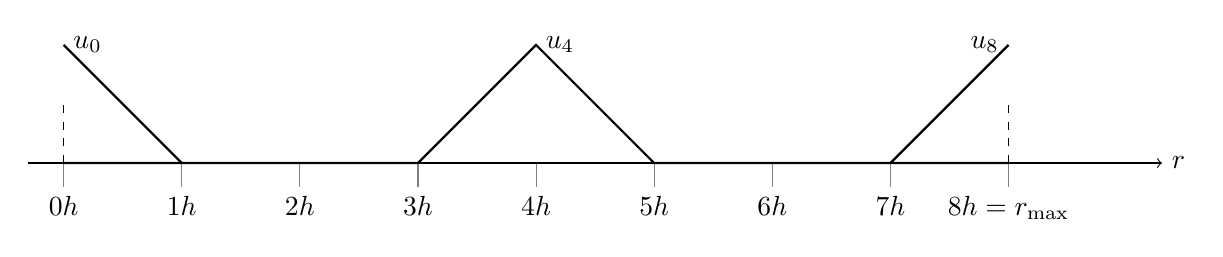
\begin{tikzpicture}[scale=1.5]

        \newcommand{\N}{8}
        \foreach \x in {0,...,\N} {
            \draw[gray] (\x,0) -- (\x,-0.2);
            \ifnum\x=\N
                \node[below] at (\x,-0.2) {$\N h = r_\text{max}$};
            \else
                \node[below] at (\x,-0.2) {$\x h$};
            \fi
        }
        \draw[dashed] (0,0) -- (0,0.5);
        \draw[dashed] (\N,0) -- (\N,0.5);

        % \draw[gray] (0,0) -- (0,0.2);
        % \node[above] at (0,0.2) {$0$};
        
        % \draw[gray] (1,0) -- (1,0.2);
        % \node[above] at (1,0.2) {$h$};
        
        % \draw[gray] (2,0) -- (2,0.2);
        % \node[above] at (2,0.2) {$2h$};
        
        % \draw[gray] (3,0) -- (3,0.2);
        % \node[above] at (3,0.2) {$3h$};
        
        \newcommand{\K}{4}
        \draw[thick] (0,0) -- (\K-1,0) -- (\K,1.0) -- (\K+1,0) -- (\N,0);
        \node at (4,1) [right] {$u_4$};

        \draw[thick] (0,1) -- (1,0);
        \draw[thick] (7,0) -- (8,1);
        \node at (0,1) [right] {$u_0$};
        \node at (8,1) [left] {$u_8$};
             

        % Axis arrow
        \draw[->] (-0.3,0) -- (\N+1.3,0) node[right] {$r$};

    \end{tikzpicture}
    \caption{Finite element method hat function. Special cases at boundaries shown. The value at the peak is $1$.}
    \label{fig:fem-basis}
\end{figure}






\section{Finite difference method}


The finite difference method differs from the finite element method in that it
does not start with a variational formulation. Instead, it starts with a grid and a collocation idea, i.e., that the unknown function is assumed to be exactly known at the grid. The derivative operators are replaced by difference formulas, and potential terms become diagonal operators using collocation.

In our 2d probolem, we need a dicretization of the radial Laplacian,
\begin{equation}
    L_0 = \frac{1}{r} \frac{\partial}{\partial r} \left( r \frac{\partial}{\partial r} \right).
\end{equation}
The basic recipe to obtain a finite difference approximation is to define a central difference $\delta_h$ of total width $h$ and replace verbatim in $L_r$, i.e.,
\begin{equation}
    \delta_h f(x) = \frac{f(x+h/2) - f(x-h/2)}{h}.
\end{equation}
Applicaton of $\delta_h$ \emph{once} gives a result living ``off-grid'' so to speak, but application twice gives a 3-point formula of grid evaluation only. In our case,
\begin{equation}
    \delta_h f(r) = h^{-1}[f(r+h/2) - f(r-h/2)]
\end{equation}
\begin{equation}
    r \delta_h f(r) = h^{-1} r [f(r+h/2) - f(r-h/2)]
\end{equation}
\begin{equation}
    L_{0,h} = r^{-1} \delta_h r \delta_h f(r) = h^{-2} r^{-1} \{ (r+h/2) [f(r+h) - f(r)] - (r-h/2) [f(r) - f(r-h)] \}.
\end{equation}
This defines the finite difference approximation of $L_0$. Its matrix is readily obtained.

It is now interesting to observe, that this finite difference approximation is \emph{identical} to the FEM approximation described above! Since the FEM basis functions are piecewise linear, their derivatives are exactly given by the finite difference formula,
\begin{equation}
    u_k'(r_k + h/2) = \delta_h u_k(r_k + h/2).
\end{equation}
Since the derivatives are piecewise constant, $t_0(u_k,u_l)$ is the integral of a piecewise \emph{linear} function due to the volume element $r dr$. This function is exactly integrated by the trapezoidal rule,
\begin{equation}
    \int_{x_k}^{x_{k+1}} f(x) \; dx = \frac{h}{2} [f(x_k) + f(x_{k+1})].
\end{equation}
When $f(x)$ is linear over the interval, the trapezoidal rule is exact.

Define $a_{kl}^j$ as the value of $u'_k(r) u'_j(r)$ inside the interval $[r_j,r_{j+1}]$, a constant. In particular, it is the value at $r_j+h/2$. Then,
\begin{equation}
    2t_0(u_k,u_{l}) = \int u_k'(r) u_l'(r) r \; dr = \sum_{j=0}^{n} a_{kl}^{j} \int_{r_j}^{r_{j+1}} r dr  = \sum_{j=0}^{n} a_{kl}^j (r_j + h/2) = \sum_{j=0}^{n} \delta_h u_k(r + h/2) \delta_h u_l(r + h/2) \cdot (r + h/2).
\end{equation}
For grid functions $f(x_j)$ and $g(x_j)$, the latter formula is equivalent to
\begin{equation}
    \sum_{j=0}^{n} h^{-2} (f_{j+1} - f_j) (g_{j+1}- g_j) (r_j + 1/2) = \sum_{j=0}^{n} h^{-2} (\delta_h^+ f)_j (\delta_h^+ g)_j \bar{r}_j,
\end{equation}
where we defined the \emph{forward} difference $\delta_h^+$, and the mean value $\bar{f}_j = (f_j + f_{j+1})/2$.
The forward difference is a linear operator on the space of grid functions, and its transpose matrix, up to boundary terms, the backward difference operator $\delta_h^-$,
\begin{equation}
    [(\delta_h^+)^T f]_j = - [\delta^- f]_j.
\end{equation}
We get,
\begin{equation}
    \sum_{j=0}^{n} h^{-2} (f_{j+1} - f_j) (g_{j+1}- g_j) (r_j + 1/2) = -\sum_{j=0}^{n} f_j (\delta_h^- \bar{R} \delta_h^+ g)_j,
\end{equation}
where $\bar{R}$ is the diagonal matrix with elements $\bar{r}_j$.

Thus, we obtain an operator $-\delta_h^- \bar{R} \delta_h^+$, and this is precisely the finite difference scheme for $L_0$.


\section{Analytical results}

We compute the kinetic energy matrix. We let $u_j(r)$ be a piecewise linear FEM basis function. For $j=0$ and $j=n+1$, the function is nonzero only on the interval $[0,h]$ and $[r_\text{max}-h,r_\text{max}]$, respectively. Otherwise, the function is nonzero on the interval $[r_{j-1},r_{j+1}]$. We note that the function is continuous, and that the derivative is constant on each interval. The derivative is given by the forward difference formula,
\begin{equation}
    u_j'(r) = \begin{cases}
        h^{-1} & r_{j-1} \leq r \leq r_j, \\
        -h^{-1} & r_j \leq r \leq r_{j+1}, \\
        0 & \text{otherwise}.
    \end{cases}
\end{equation}

\subsection{Mass matrix diagonal elements}

We begin with the mass matrix. We have
\begin{equation}
    \mathsf{S}_{k,l} = \braket{u_k,u_l}_r = \int_0^{r_\text{max}} u_k(r) u_l(r) r \; dr.    
\end{equation}
For $k=l$, and $k$ an inner grid point, we have
\begin{align}
    \mathsf{S}_{k,k} &= \int_{r_{k-1}}^{r_{k+1}} u_k(r)^2 r \; dr \\
    &= \int_{r_{k-1}}^{r_k} ((r-r_{k-1}) h^{-1})^2 r dr + \int_{r_k}^{r_{k+1}} (1 - h^{-1}(r - r_{k}))^2 r dr \\
    &= \int_0^h (h^{-1} r)^2 (r + r_{k-1}) dr + \int_0^h (1 - h^{-1} r)^2 (r + r_{k}) dr \\
    &= h^{-2} \int_0^h (r^3 + r_{k-1} r^2) dr + h^{-2} \int_0^h (h^2 + r^2 - 2 hr)(r + r_k) dr   \\
    &= h^{-2} [ \frac{1}{4} h^4 + \frac{1}{3} r_{k-1} h^3] + h^{-2} \int_0^h (rh^2 + r^3 - 2hr^2 + h^2 r_k + r^2 r_k - 2hr r_k) dr \\
    &= h^{-2} [ \frac{1}{4} h^4 + \frac{1}{3} r_{k-1} h^3] 
    + h^{-2} [ \frac{1}{2}h^4 + \frac{1}{4} h^4 - \frac{2}{3} h^4 + h^3 r_k + \frac{1}{3} h^3 r_k - h^3 r_k ] \\
    & = \frac{1}{3} h^2 + \frac{1}{3} h r_{k-1} + \frac{1}{3} h r_k .
\end{align}
For symmetry, it is better to express this in terms of $r_k$ only. We have
\begin{equation}
    \mathsf{S}_{k,k} = \frac{1}{3} h^2 + \frac{1}{3} h (r_k - h) + \frac{1}{3} h r_k  = \frac{1}{3} h^2 + \frac{2}{3} h r_k - \frac{1}{3} h^2 = \frac{2}{3} h r_k.
\end{equation}
For $k=0$, only the second integral contributes, and we get
\begin{equation}
    \mathsf{S}_{0,0} = \int_0^h (1 - h^{-1} r)^2 r dr = \frac{1}{3} h^2.
\end{equation}

For $k=n+1$, only the first integral contributes, and we get
\begin{equation}
    \mathsf{S}_{n+1,n+1} = \frac{1}{4} h^2 + \frac{1}{3} (r_\text{max}-h) h
 = \frac{1}{4} h^2 + \frac{1}{3} r_\text{max} h - \frac{1}{3} h^2 = \frac{1}{3} r_\text{max} h + \frac{1}{12} h^2.
\end{equation}


\section{Time-dependent Hartree--Fock on a grid}

In this section, we consider the task of propagating the Hartree--Fock state when the orbitals are defined on a grid.

The contiuous  RHF Fock operator is a \emph{linear operator} that \emph{depends on the occupied orbitals $\varphi_i$}. The action on an arbitrary $\psi$ is
\begin{equation}
    \hat{f} \psi = \hat{h} \psi +  \left( 2 \hat{j} - \hat{k} \right) \psi,
\end{equation}
where
\begin{equation}
    \hat{h} = -\frac{1}{2} \nabla^2 - V(r),
\end{equation}
with $V(r)$ the nuclear potential, and
where the Hartree potential $\hat{j}$ is 
\begin{equation}
    [\hat{j} \psi](r) = \psi(r) \sum_j \int \frac{\varphi_j^*(r') \varphi_j(r')}{|r-r'|} \; dr,
\end{equation}
and the exchange potential $\hat{k}$ is
\begin{equation}
    [\hat{k} \psi](r) = \sum_j \varphi_j(r) \int \frac{\varphi_j^*(r') \psi(r')}{|r-r'|} \; dr.
\end{equation}
We now introduce a discretization, which we generically assume is of collocation type: $\psi(r)$ are the pointwise values on of a wavefunction on a set of nodes, and $\hat{h}$ correspondingly interpreted as mapping from grid values to grid values as well. The Hartree and exchange potentials become diagonal operators, and we introduce some approximation $\hat{W}$ that takes a discrete density and returns a discrete potential, 
\begin{equation}
    \hat{W}[\rho](r) \approx \int \frac{\rho(r')}{|r-r'|} \; dr.
\end{equation}
This is then a discrete solution of the Poisson equation $\nabla^2 \hat{W}[\rho] = -4 \pi \rho$ with proper boundary conditions.

We now get the discrete Fock operator,
\begin{equation}
    \hat{f} \psi = \hat{h} \psi +  \left( 2 \hat{W}[\sum_j \varphi_j\varphi_j^*] - \sum_j \hat{W}[\psi \varphi_j^*] \right) \psi,
\end{equation}
where the sum is over the occupied orbitals. The time-dependent Hartree--Fock equation is then
\begin{equation}
    i \partial_t \varphi_j = \hat{f} \varphi_j,
\end{equation}
which is to hold for all occupied orbitals $\varphi_j$.

In HF theory the unknown is a vector of orbitals, and the Fock operator is a block operator acting on this vector. We will now derive the form of the Fock operator in the grid representation.

We introduce a compound wavefunction $\Phi = (\varphi_1,\ldots,\varphi_n)$, where we imagine each orbital as a vector, and $\Phi$ being these vectors stacked on top of each other. Thus, if we have $M$ orbitals, and each orbital is of dimension $n$, then $\Psi$ consists of $M$ blocks of length $n$. the operators that we will consider acting on $\Phi$ are then block matrices. The vector $\Phi$ is one particular element, consisting of the actual orbitals, of the compound vector space. We will denote a genera element of this vector space as $\Psi$, and its components are \emph{not} necessarily the orbitals,
\begin{equation}
    \Psi = (\psi_1,\ldots,\psi_M).
\end{equation}
We introduce a projection operator $P_j$ that projects onto the $j$th component,
\begin{equation}
    P_j \Psi = \psi_j.
\end{equation}
The formal adjoint of this operator takes an orbital and inserts in into a compound wavefunction,
\begin{equation}
    P_i^\dag \psi = (0_{j=0}, \ldots, 0_{j=i-1}, \psi, 0_{j=i+1},\ldots, 0_{M}).
\end{equation}
For any single-orbital operator $\hat{a}$ we note that $P_i^\dag \hat{a} P_j$ is a block matrix being all zero except for the block located at position $ij$ which becomes $\hat{a}$.

We wish to identify the nonlinear block operator $\hat{F}$ acting on $\Psi$, which must satisfy
\begin{equation}
    \hat{F} \Psi = \sum_i P_i^\dag \hat{f} P_i \Psi.
\end{equation}
The linear parts of $\hat{F}$ will be unique, while the nonlinear parts can be written in a variety of ways, as we will see.

Let us first consider the block operator corresponding to $\hat{h}$. We get
\begin{equation}
    \hat{H} = \sum_i P_i^\dag \hat{h} P_i = \blockdiag(\hat{h},\ldots,\hat{h}),
\end{equation}
where the right hand side is a block diagonal matrix with diagonal blocks equal to $\hat{h}$.

We next consider the Hartree potential terms: 
\begin{equation}
    \hat{j} P_i \Psi = \sum_j \hat{W}[\varphi_j \varphi_j^*] P_j\Psi = \sum_j \hat{W}[(P_j \Phi) (P_j\Phi)^*] P_i \Psi.
\end{equation}
Thus,
\begin{equation}
    \hat{J} = \sum_{ij} P_i^\dag \hat{W}[(P_j \Phi) (P_j\Phi)^*]  P_i.
\end{equation}
Similarly,
\begin{equation}
    \hat{k} P_i \Psi = \sum_j \hat{W}[(P_i\Psi) \varphi_j^*] \varphi_j = \sum_j \hat{W}[(P_i \Psi) (P_j\Phi)^*] P_i \Phi.
\end{equation}
Thus,
\begin{equation}
    \hat{K} = \sum_{ij} P_i^\dag \hat{W}[(P_i \; \cdot\; ) (P_j\Phi)^*]  P_j\Phi.
\end{equation}
We get for the total Fock operator
\begin{equation}
    \hat{F}(\Phi) = \hat{H} + 2 \sum_{ij} P_i^\dag \hat{W}[(P_j \Phi) (P_j\Phi)^*]  P_i - \sum_{ij} P_i^\dag \hat{W}[(P_i \; \cdot\; ) (P_j\Phi)^*]  P_j \Phi.
\end{equation}
We recall that $\hat{f}$ is a linear operator that depends on the RHF orbitals. Similarly, $\hat{F}(\Phi)$ is still a linear operator that depdends on $\Phi$. We now apply $\hat{F}(\Phi)$ to $\Phi$ in particular and observe something interesting:
\begin{equation}
    \hat{F}(\Phi) \Phi = \hat{H} \Phi + 2 \sum_{ij} P_i^\dag \hat{W}[(P_j \Phi) (P_j\Phi)^*]  P_i \Phi - \sum_{ij} P_i^\dag \hat{W}[(P_i \Phi ) (P_j\Phi)^*]  P_j\Phi.
\end{equation}
From this, we can extract a \emph{different} nonlinear operator $\hat{F}'(\Phi)$:
\begin{equation}
    \hat{F}'(\Phi) = \hat{H} + 2 \sum_{ij} P_i^\dag \hat{W}[(P_j \Phi) (P_j\Phi)^*]  P_i - \sum_{ij} P_i^\dag \hat{W}[(P_i \Phi ) (P_j\Phi)^*]  P_j.
\end{equation}
This operator is such that 
\begin{equation}
    \hat{F}'(\Phi) \Phi = \hat{F}(\Phi) \Phi,
\end{equation}
but in general we have
\begin{equation}
    \hat{F}'(\Phi) \Psi \neq \hat{F}(\Phi) \Psi.
\end{equation}
So as linear operators they are actually different. The point is that in $\hat{F}'$ we isolate the nonlinearity completely inside the mean-field operators $\hat{W}$.

We now consider the time-dependent Hartree--Fock equation. We have
\begin{equation}
    i \partial_t \varphi_j = \hat{f}(\varphi_1,\cdots,\varphi_M) \varphi_j,
\end{equation}
This translates to
\begin{equation}
    i \partial_t \Phi = \hat{F}(\Phi) \Phi = \hat{F}'(\Phi)\Phi.
\end{equation}
We can now define a constant mean-field (CMF) class of methods: Over an interval $[t, t+\Delta t]$ we approximate the time-dependent $\Phi(t+s) = \bar{\Phi}(t)$ \emph{inside the mean-field terms}. Over the time interval we thus have,
\begin{equation}
    i \partial_t \Phi = \hat{F}'(\bar{\Phi}) \Phi.
\end{equation}
This is a linear equation. However, whereas $\hat{H}$ and $\hat{J}$ are block diagonal, the total $F'(\bar{\Phi})$ is not. Indeed, we see that the blocks of $\hat{F}'(\bar{\Phi})$ are given by 
\begin{equation}
    \hat{F}'_{ij}(\bar{\Phi}) = \delta_{ij} \left(\hat{h} + 2 \hat{W}[(\sum_k P_j \bar{\Phi}) (P_j\bar{\Phi})^*] \right) -  \hat{W}[(P_i \bar{\Phi} ) (P_j\bar{\Phi})^*] .
\end{equation}
Thus, the linear operator $\hat{F}'(\bar{\Phi})$ couples the different blocks of $\Phi$. However, the off-diagonal blocks are all diagonal operators, and the diagonal blocks are 
\begin{equation}
    \hat{h}_{\text{eff}} = \hat{t} + \hat{v} + \hat{v}_J,
\end{equation}
with $\hat{v}_J = \hat{W}[\sum_j |\bar{\varphi}_j|^2]$ being a potential.

I suggest to do a splitting scheme: We write the propagator from $t$ to $t + \Delta t$ as
\begin{equation}
    \begin{split}
    \mathcal{U} &= \exp[-i\Delta t \hat{F}'(\bar{\Phi})] = \exp[ -i \Delta t (\hat{H}_\text{eff} - \hat{K}'(\bar{\Phi}))] \\ &= \exp[i\Delta t \hat{K}'(\bar{\Phi})/2] \exp[-i\Delta t \hat{H}_\text{eff}] \exp[i\Delta t \hat{K}'(\bar{\Phi})/2] + \mathcal{O}(\Delta t^3).
    \end{split}
\end{equation}
Since $\hat{H}_\text{eff}$ is block diagonal,
\begin{equation}
    \exp[-i\Delta t \hat{H}_\text{eff}] = \blockdiag(\exp[-i\Delta t \hat{h}_\text{eff}],\ldots,\exp[-i\Delta t \hat{h}_\text{eff}]),
\end{equation}
that is, each block is a propagator for a single orbital with a modified potential.

The operator $\hat{K}'(\bar{\Phi})$ is a block operator, and its exponential is equivalent to solving the TDSE
\begin{equation}
    i \partial_t \Phi = -\hat{K}'(\bar{\Phi}) \Phi,
\end{equation}
over a time interval of length $\Delta t$. We observe that the ``Hamiltonian'' here is just the exchange potential, a diagonal matrix with eigeenvalues whose absolute values are bounded by the values of the exchange potential elements. In particular, these eigenvalues are \emph{bounded uniformly} as our discretization becomes finer. \emph{Explicit RK methods can be used to solve this equation.} We also note that the action of $\hat{K}'(\bar{\Phi})$ on a vector $\Psi$ is rather efficient, as the blocks are diagonal. Selecting an RK method for this, we can use plain RK4, but this is slightly more costly than needed. We can also use, say, the classical third order scheme got $y' = f(t,y)$:
\begin{enumerate}
\item Calculate \(k_1 = f(t_n, y_n)\).
\item Calculate \(k_2 = f\left(t_n + \frac{1}{2}\Delta t, y_n + \frac{1}{2}\Delta t k_1\right)\).
\item Calculate \(k_3 = f(t_n + \Delta t, y_n - \Delta t k_1 + 2\Delta t k_2)\).
\item Update \(y_{n+1} = y_n + \frac{\Delta t}{6}(k_1 + 4k_2 + k_3)\).
\end{enumerate}




\end{document}
